\documentclass[12pt]{article}
\usepackage[margin=1in]{geometry}
\geometry{letterpaper}                  
\usepackage{graphicx}
\usepackage[hyphens]{url}
\usepackage{fancyhdr}
%\pagestyle{fancy}
\usepackage{fixltx2e}
\usepackage{amsmath,amsfonts,amsthm,amssymb}
\usepackage{graphicx}
\usepackage{algorithm}
\usepackage{algorithmic}
\usepackage{url}
\usepackage[normalem]{ulem}
\usepackage[pdftex]{color}
\usepackage{varioref}
\usepackage{mathrsfs}
\usepackage{amsmath}
\labelformat{equation}{\textup{(#1)}}
\usepackage[sort&compress,colon,square,numbers]{natbib}
%\usepackage{cite}


\usepackage{color}
\newcommand{\todo}[1]{{\color{red}{\it TODO: #1}}}
\newcommand{\jovo}[1]{{\color{green}{\it jovo: #1}}}
\newcommand{\will}[1]{{\color{blue}{\it will: #1}}}
\newcommand{\greg}[1]{{\color{cyan}{\it greg: #1}}}

\DeclareMathOperator*{\argmin}{arg\,min}


\begin{document}

\begin{center}\Large \bf EN.580.694: Statistical Connectomics \\ Final Project Report \end{center}
\begin{center} Elan Hourticolon-Retzler $\cdot$  \today \end{center}
\bigskip


\subsection*{Extending FAQ Graph Matching to use Anti-Seed Informating}
$\\ \\$
\centerline{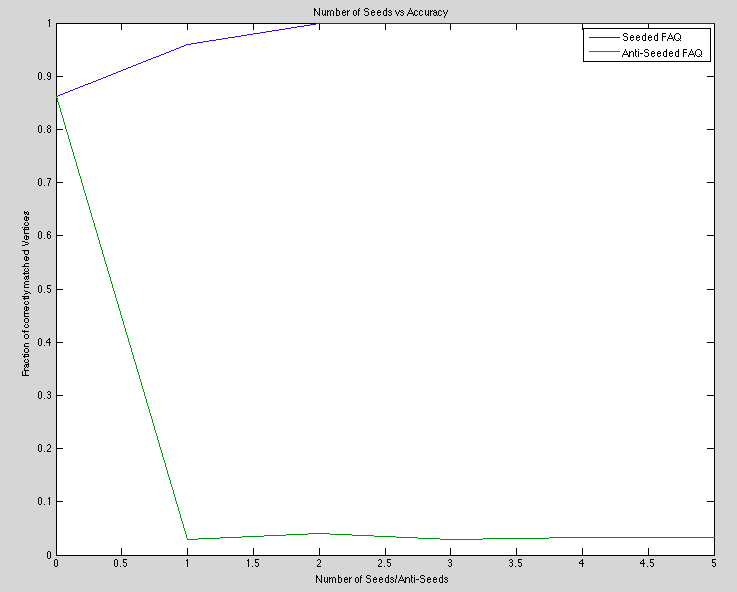
\includegraphics[scale=0.5]{results.png}}
\newpage

\paragraph{Opportunity}

Fast Approximate Quadratic Programming for Graph Matching has proven itself to be an effective method for graph matching, finding the best permutation matrix to map the vertices of one graph to another. This is done by relaxing the objective function (of minimizing edge differences between graphs) and using an iterative approach to find an optimal permutation matrix.

Fishkind,  Adali, and  Prieb have additionally demonstrated that first seeding even just a few vertex matches greatly improves performance. This was done by breaking our Permutation matrix into blocks and leaving us with a smaller subset of vertices that we need to match.


\paragraph{Challenge}

Since we know that adding information about positive matches to our algorithm is useful it is conceivable that adding information about which vertices would similarly be helpful since it has the same effect of reducing our search space - albeit each anti seed being largely less informative since each Seed immediately implies NumVertices-1 AntiSeeds . Another impetus is that finding and annotation positive matches can be a costly process however it may be much 

\paragraph{Action}
%Test-retest (TRT) reliability is a measure which seeks to compare connectomes estimated for the same subject across different scans to the remainder of the dataset. A successful TRT test results in the same subject graphs being more similar to one another than all other graphs. Here, we employed Test-ReTest (TRT) reliability in order to evaluate the performance of four commonly used atlases; Desikan \cite{desikan}; Harvard-Oxford \cite{harvardoxford}; Juelich \cite{juelich}; Talairach \cite{talairach}.

In a similar fashion of Fishkind,  Adali, and  Prieb, I  broke up the permutation matrix into blocks however instead of marking known matches with the identity matrix sized according to the number of seeds I used a block of 0's sized based on the number of anti-seeds. 

From this I proceeded with the same relaxation of the constraints requiring P to be permutation matrix - from each element being $\{0,1\}$ to each element lying in the range $[0,1]$.

Since the both the authors of the FAQ paper and the Seeded variant (Priebe and Vogelstein) paper open sourced their code I was able to build on it changing the Permutation matrix and associated gradients.

\paragraph{Resolution}
%Shown above is the TRT result for each atlas using graphs from the KKI2009 dataset. We can see here that with the provided graphs, the Desikan and Harvard-Oxford atlases correctly match $41$ of $42$ scans and have $70$ and $48$ regions, respectively. The Juelich and Talairach atlases both correctly matched all subjects and have $121$ and $1106$ regions, respectively. It can also be seen that the Talairach atlas has much higher discrimination across subjects than the other three atlases, as indicated by the larger dynamic range of image intensities. This suggests that parcelation schemes with too few regions may discard useful information about the brain graphs.

Despite my efforts at changing my formulation to include Anti-Seeds, performance has significantly suffered. My original thoughts let me to suspect a bug in my code or a error in my calculations when calculating the different block gradients, however reviewing both has turned up nothing. I now suspect there is a fundamental inconsistency in how I'm approaching the problem (i.e. how I'm partitioning the permutation matrix) since adding even a single Anti-Seed is drastically affecting my results.

\paragraph{Future Work}
%Moving forward, it we will evaluate whether or not specific atlas region labels matter when performing comparing graphs, or rather the scale/number of regions. Randomly permuted atlases could be generated over a large range of scales and a peak operating point determined. This information can aide in building better, more interpretable classifiers for inference and diagnosis.

This project is very much a work in progress in that I believe it to be a worthwhile and achievable endeavor however my current efforts have turned out to be fruitless.

Immediate future work includes discovering why introducing Anti-Seeds is so significantly derailing performance. 

After that issue is solved I'd like to move away from large block Anti-Seeds towards finer grain resolution (ie. breaking up Anti-Seeds into many disjoin blocks instead of a sing large one).  The reason I did not initially start with this is that automatically partitioning the permutation matrix in this way seems to be a rather nontrivial programatic undertaking, one that can be pursued once I have the simplest case working). 
\nocite{*}

\bibliography{statconn.bib}
\bibliographystyle{plain}


\end{document}  















